% ! TeX root = ../../master-thesis.tex

\section{Step Simulator}
\label{section:implementation:step-simulator}

The implementation of a step simulator is represented by the class diagram in
Figure \ref{figure:step-simulator-class-diagram}, which is based on the design
described in Section \ref{section:design:step-simulation}.

\begin{figure}[!ht]
  \centering
  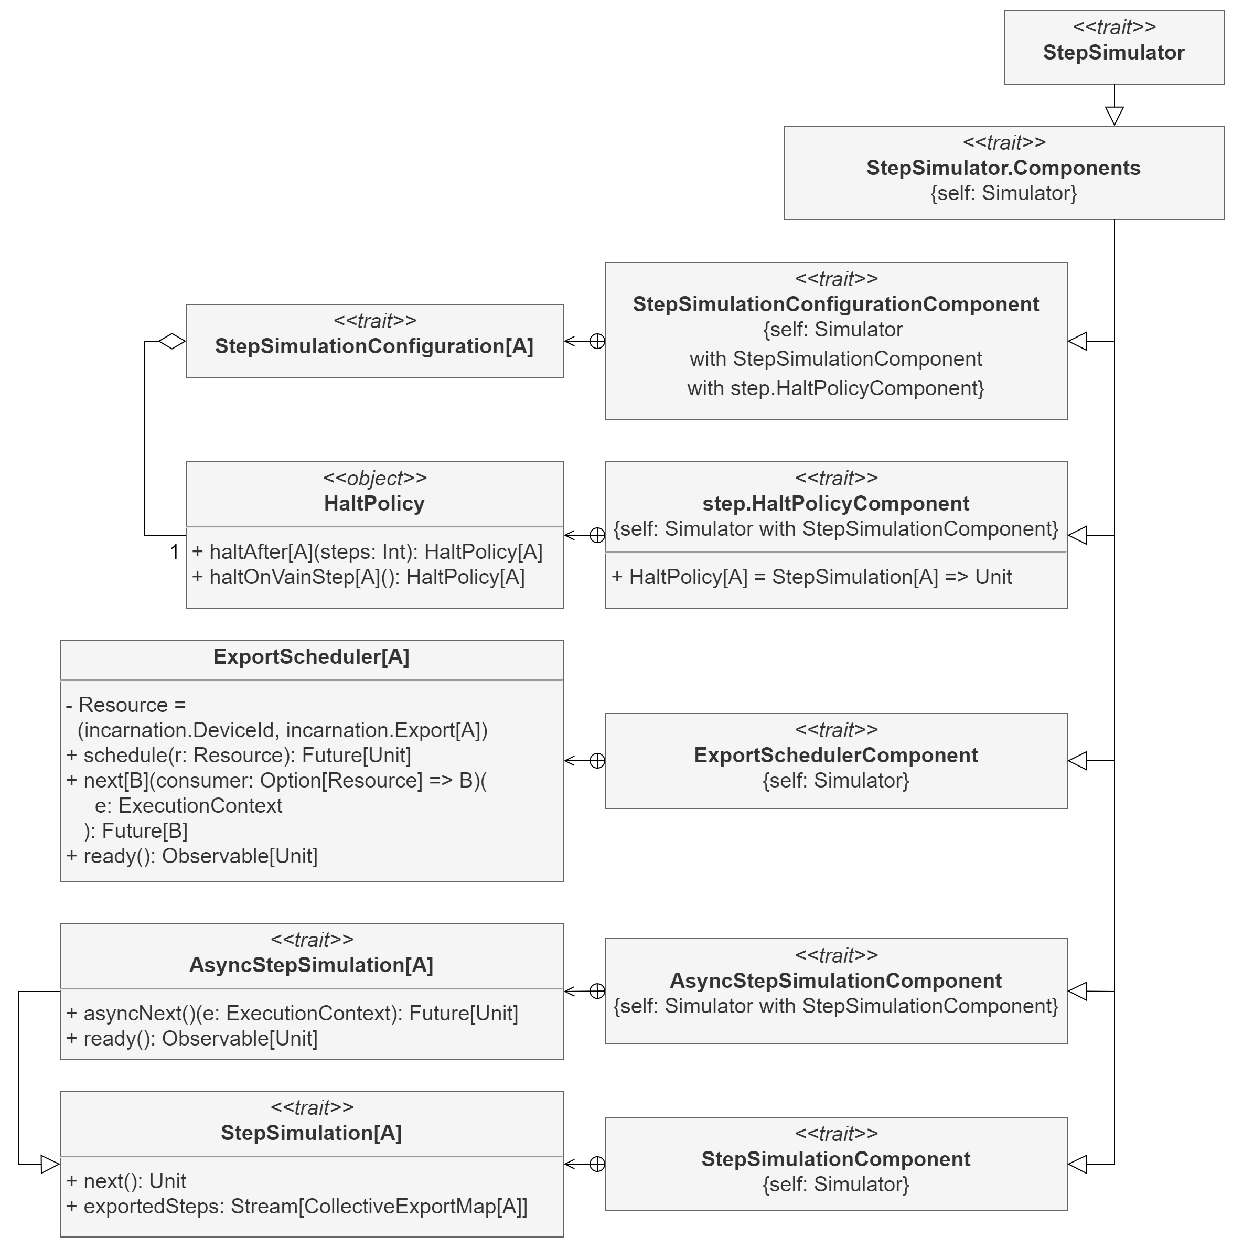
\includegraphics[width=1\textwidth]{resources/figures/diagrams/short/step-simulator-class-diagram.pdf}
  \caption[A UML class diagram of the step simulator]{
    A UML class diagram of the step simulator and its components.
  }
  \label{figure:step-simulator-class-diagram}
\end{figure}

A \texttt{StepSimulator} is a \texttt{Simulator} that creates
\texttt{StepSimulation}s. As per design, a \texttt{StepSimulation} provides
enhanced observability and controllability by means of the methods
\texttt{next}, which executes a step of the simulation by transmitting the next
device export to the neighbors and the user, and \texttt{exportedSteps}, which
supplies a \texttt{Stream} of the device exports transmitted at each step.

A thread-safe variant of \texttt{StepSimulation} is the
\texttt{AsyncStepSimulation}, which provides a new method \texttt{asyncNext},
executing the next step of the simulation in a given \texttt{ExecutionContext},
and a new property \texttt{ready}, allowing registering callbacks to execute
each time a new export is available for transmission. Actually, only an
implementation of \texttt{AsyncStepSimulation} has been developed at the
moment, meaning that every \texttt{StepSimulation} is an
\texttt{AsyncStepSimulation} under the hood. In the future, a specific
implementation of \texttt{StepSimulation} may be developed to be optimized for
single-threaded execution.

Specifically, the implemented \texttt{AsyncStepSimulation} involves keeping
track of the device exports through per-device queues, deferring their
transmission to the neighbors until requested by the user, that is when the
methods \texttt{next} or \texttt{asyncNext} are called, which delegate the
propagation of change to the user or to an \texttt{ExecutionContext}
respectively. The device queues are managed by an \texttt{ExportScheduler}:
each time an export is produced, the method \texttt{schedule} of the scheduler
is called, queuing the device export for later consumption; each time the next
step of the simulation is requested by the user, the method \texttt{next} of
the scheduler is called, dequeuing and transmitting the next export both to the
neighbors and the user. The transmission to the user happens by pushing the
exports into the \texttt{exportedSteps} stream. If all the device queues are
empty, an empty event is pushed instead.

The \texttt{ExportScheduler} decides the order of transmission of the device
exports, preserving the order of computation for each device (i.e., the export
of a device cannot be transmitted before its previous export). In particular,
the scheduling policy adopted by the current implementation is a best-effort
round-robin, in which each device is given the same chance to transmit its
exports as long as they have some to transmit, guaranteeing fairness during the
simulation.

The \texttt{SimulationConfiguration} of a \texttt{StepSimulation} is modeled by
the class \texttt{StepSimulationConfiguration}. In addition to the
\texttt{Environment}, the configuration includes an \texttt{HaltPolicy}, which
contains the logic for determining the end of the simulation. Some built-in
\texttt{HaltPolicy}s are already defined in the corresponding simulator
component, namely: \texttt{never}, which never halts the simulation (the user
may still stop it at any time); \texttt{haltWhen}, which halts the simulation
when a given predicate holds for the state of the aggregate;
\texttt{halt\-After}, which halts the simulation after a given number of steps;
finally, \texttt{haltOnVainStep}, which halts the simulation when a step is
executed, but all the export queues are empty. Additionally,
\texttt{HaltPolicy}s may be merged by means of the \texttt{combine} operator to
consider multiple conditions of termination, halting the simulation when any of
them is satisfied.

The \texttt{StepSimulationConfiguration} is interpreted by the
\texttt{StepSimulation} when the \texttt{start} method is called, creating the
devices of the aggregate, building its computational graph, scheduling the
first exports and setting up the \texttt{HaltPolicy}.

\paragraph{Example.}
A practical application of the \texttt{StepSimulator} is demonstrated in the
following program (Listing \ref{listing:step-simulator-example}).

\lstinputlisting[
  language=Scala,
  caption={
      [An application of the step simulator]
      An application of \texttt{StepSimulator}. The simulator is used to
      display the device exports on the standard output.
    },
  captionpos=b,
  label={listing:step-simulator-example}
]{resources/listings/step-simulator-example.txt}
